
%%%%%%%%%%%%%%%%%%%%%%%%%%%%% Define Article %%%%%%%%%%%%%%%%%%%%%%%%%%%%%%%%%%
\documentclass[conference]{IEEEtran}
%%%%%%%%%%%%%%%%%%%%%%%%%%%%%%%%%%%%%%%%%%%%%%%%%%%%%%%%%%%%%%%%%%%%%%%%%%%%%%%

%%%%%%%%%%%%%%%%%%%%%%%%%%%%% Using Packages %%%%%%%%%%%%%%%%%%%%%%%%%%%%%%%%%%
\usepackage{geometry}
\usepackage{graphicx}
\usepackage{amssymb}
\usepackage{amsmath}
\usepackage{amsthm}
    
\usepackage{empheq}
\usepackage{mdframed}
\usepackage{booktabs}
\usepackage{lipsum}
\usepackage{graphicx}
\usepackage{color}
\usepackage{psfrag}
\usepackage{pgfplots}
\usepackage{bm}
\usepackage[spanish]{babel}
\usepackage[utf8]{inputenc} % Codificación UTF-8
\usepackage{amsmath}        % Soporte para ecuaciones matemáticas
\usepackage{graphicx}       % Manejo de imágenes
\usepackage{hyperref}       % Hipervínculos
\usepackage{caption}        % Formato para figuras
\usepackage{multirow}
\usepackage{subcaption}
\usepackage{biblatex}
\usepackage{csquotes}
\usepackage{bookmark}
%%%%%%%%%%%%%%%%%%%%%%%%%%%%%%%%%%%%%%%%%%%%%%%%%%%%%%%%%%%%%%%%%%%%%%%%%%%%%%%

% Other Settings

%%%%%%%%%%%%%%%%%%%%%%%%%% Page Setting %%%%%%%%%%%%%%%%%%%%%%%%%%%%%%%%%%%%%%%
\geometry{a4paper, margin=1in}

%%%%%%%%%%%%%%%%%%%%%%%%%% Define some useful colors %%%%%%%%%%%%%%%%%%%%%%%%%%
\definecolor{ocre}{RGB}{243,102,25}
\definecolor{mygray}{RGB}{243,243,244}
\definecolor{deepGreen}{RGB}{26,111,0}
\definecolor{shallowGreen}{RGB}{235,255,255}
\definecolor{deepBlue}{RGB}{61,124,222}
\definecolor{shallowBlue}{RGB}{235,249,255}
%%%%%%%%%%%%%%%%%%%%%%%%%%%%%%%%%%%%%%%%%%%%%%%%%%%%%%%%%%%%%%%%%%%%%%%%%%%%%%%

%%%%%%%%%%%%%%%%%%%%%%%%%% Define an orangebox command %%%%%%%%%%%%%%%%%%%%%%%%
\newcommand\orangebox[1]{\fcolorbox{ocre}{mygray}{\hspace{1em}#1\hspace{1em}}}
%%%%%%%%%%%%%%%%%%%%%%%%%%%%%%%%%%%%%%%%%%%%%%%%%%%%%%%%%%%%%%%%%%%%%%%%%%%%%%%

%%%%%%%%%%%%%%%%%%%%%%%%%%%% English Environments %%%%%%%%%%%%%%%%%%%%%%%%%%%%%
\newtheoremstyle{mytheoremstyle}{3pt}{3pt}{\normalfont}{0cm}{\rmfamily\bfseries}{}{1em}{{\color{black}\thmname{#1}~\thmnumber{#2}}\thmnote{\,--\,#3}}
\newtheoremstyle{myproblemstyle}{3pt}{3pt}{\normalfont}{0cm}{\rmfamily\bfseries}{}{1em}{{\color{black}\thmname{#1}~\thmnumber{#2}}\thmnote{\,--\,#3}}
\theoremstyle{mytheoremstyle}
\newmdtheoremenv[linewidth=1pt,backgroundcolor=shallowGreen,linecolor=deepGreen,leftmargin=0pt,innerleftmargin=20pt,innerrightmargin=20pt,]{theorem}{Theorem}[section]
\theoremstyle{mytheoremstyle}
\newmdtheoremenv[linewidth=1pt,backgroundcolor=shallowBlue,linecolor=deepBlue,leftmargin=0pt,innerleftmargin=20pt,innerrightmargin=20pt,]{definition}{Definition}[section]
\theoremstyle{myproblemstyle}
\newmdtheoremenv[linecolor=black,leftmargin=0pt,innerleftmargin=10pt,innerrightmargin=10pt,]{problem}{Problem}[section]
%%%%%%%%%%%%%%%%%%%%%%%%%%%%%%%%%%%%%%%%%%%%%%%%%%%%%%%%%%%%%%%%%%%%%%%%%%%%%%%

%%%%%%%%%%%%%%%%%%%%%%%%%%%%%%% Plotting Settings %%%%%%%%%%%%%%%%%%%%%%%%%%%%%
\usepgfplotslibrary{colorbrewer}
\pgfplotsset{width=8cm,compat=1.9}
%%%%%%%%%%%%%%%%%%%%%%%%%%%%%%%%%%%%%%%%%%%%%%%%%%%%%%%%%%%%%%%%%%%%%%%%%%%%%%%

%%%%%%%%%%%%%%%%%%%%%%%%%%%%%%% Title & Author %%%%%%%%%%%%%%%%%%%%%%%%%%%%%%%%
\author{\IEEEauthorblockN{Carlos Fernando Torres Ferrer, Daniel Fernando Aranda Contreras, Dairo Alexander Lobo Moreno,\\ Yulieth Valentina Portilla Jaimes}
\IEEEauthorblockA{Escuela E3T, Universidad Industrial de Santander\\
Correo electrónico: \{carlos2221116, daniel2221648, dairo2221123, yulieth2221136\}@correo.uis.edu.co}}
%%%%%%%%%%%%%%%%%%%%%%%%%%%%%%%%%%%%%%%%%%%%%%%%%%%%%%%%%%%%%%%%%%%%%%%%%%%%%%%
\begin{document}
% Título
\title{\uppercase{Diseño de infraestructura eléctrica de la nueva subestación Huila 230 kV y líneas de transmisión asociadas}}
\maketitle
% Resumen
% Palabras clave        
\begin{IEEEkeywords}
    Frecuencia de muestreo, Mediciones eléctricas, Análisis de señales, Valor RMS, Muestreo de señales, Errores de estimación, Parámetros del sistema eléctrico, Comparación de procesos de muestreo.   
\end{IEEEkeywords}

\section*{Introducción}
Los parámetros de diseño del proyecto se definen a partir del Anexo 1 de la convocatoria UPME, el Código de Redes (Resolución CREG 025 de 1995 y CREG 098 de 2000) y el Reglamento Técnico de Instalaciones Eléctricas (RETIE). A continuación, se resumen los principales aspectos técnicos y de diseño del proyecto.


\section{Parámetros de Diseño Según la CREG025 – 1995}
\subsection{Frecuencia}
El valor nominal de la frecuencia del SIN colombiano es de 60,00 Hz.

\subsection{Tensión}
La tensión nominal del STN es de 220 kV y 500 kV. No obstante, para efectos de diseño de nuevas instalaciones, se exige una tensión nominal de 230 kV.

\subsection{Longitud de la Línea de Transmisión}
En todas las actividades relacionadas con diseño, cálculo, tendido, estimación de materiales y construcción, se entiende que la línea de transmisión está comprendida entre los pórticos de salida de cada subestación que sirve de fijación al vano que las une a la primera torre.

\subsection{Conductores por Fase}
\begin{itemize}
    \item Resistencias eléctricas, medida en W/km a 20 grados C, debe ser igual o menor a la determinada por la UPME.
    \item Niveles de campos eléctricos y magnéticos:
    \begin{itemize}
        \item A borde de servidumbre = 5 kV/m
        \item Campo magnético = 1 Gauss
        \item Cruces de carreteras 10 a 12 kV/m
    \end{itemize}
    \item Niveles máximos de radio interferencia:
    \begin{itemize}
        \item Zonas rurales: 22 dB a 80 m del eje de la línea a 1000 kHz
        \item Zonas Urbanas: 22 dB a 40 m del eje de la línea a 1000 kHz
    \end{itemize}
    \item Cable de guarda: Todas las líneas de transmisión del STN deberán tener cable de guarda. Este deberá soportar el impacto directo de las descargas eléctricas atmosféricas.
    \item Aislamiento: Se define mediante combinación de las distancias mínimas, todo esto para evitar sobretensiones por descargas atmosféricas, de frecuencia industrial, etc.
\end{itemize}

\subsection{Comportamiento Mecánico del Conductor de Fase y Cable de Guarda}
En cualquier condición, la tensión longitudinal máxima en el conductor o cable de guarda no deberá exceder el 50\% de su correspondiente tensión de rotura.

\subsection{Estructuras}
El cálculo de estas, depende mucho del tipo de estructura, ya sea de suspensión, de retención o de terminal. También se asocian a si estos están en una condición normal o anormal, incluyendo parámetros de viento, temperatura, rotura de los conductores o cables de guarda, etc.

\subsection{Cimentaciones}
Las cimentaciones deberán resistir todas las hipótesis de carga que se estipulen para cada uno de los tipos de estructura.

\subsection{Localización de Estructuras}
La localización de las estructuras deberá cumplir con ciertos requisitos para la seguridad sobre el terreno y obstáculos, entre estos se encuentran las carreteras principales, árboles, cercas, ferrocarriles, ríos navegables, embalses, entre otros.

\subsection{Cadenas de Aisladores y Herrajes}
Los aisladores deberán ser fabricados en porcelana, vidrio o poliméricos.

\subsection{Puesta a Tierra}
Este sistema de puesta a tierra debe estar en cada estructura y ser diseñado según las condiciones específicas de las líneas.

\subsection{Servidumbres}
El ancho de la faja de servidumbre requerida será establecido por el propietario de la línea, ajustado con base en los niveles de campo electromagnético y de radio interferencia.

\section*{Aspectos Técnicos de la Convocatoria}
La subestación Huila 230 kV contará con una configuración tipo interruptor y medio, incluyendo cuatro bahías de línea y dos bahías de transformación, todas con cortes centrales. Se establecerán dos diámetros completos y dos incompletos a 230 kV, garantizando alta confiabilidad operativa y posibilidad de expansión futura mediante enlaces removibles. La subestación podrá ser de tipo convencional (AIS), aislada en gas (GIS) o una solución híbrida, según normativa aplicable. Tendrá niveles de aislamiento de 1050 kV para el impulso tipo rayo y 460 kV a frecuencia industrial. Además, dispondrá de servicios auxiliares en AC (120/208 V, tres fases, cuatro hilos) y DC (125 V).

El sistema eléctrico del proyecto operará con una tensión nominal de 230 kV, una frecuencia asignada de 60 Hz, con puesta a tierra sólida y un número de fases igual a tres (3), cumpliendo así con los estándares técnicos requeridos para el sistema de transmisión en alta tensión. Deben garantizarse sistemas de control, protecciones, medición, comunicaciones e infraestructura asociada, compatibles con la infraestructura existente.

Las líneas de transmisión del proyecto operarán a una tensión nominal de 230 kV e implican la construcción de una línea de doble circuito o dos líneas independientes desde la subestación Huila: aproximadamente 6 km hacia la línea Betania–Mirolindo, para su reconfiguración como Betania–Huila–Mirolindo, y 6 km hacia la línea Betania–Tuluní, para conformar Betania–Huila–Tuluní. El proyecto incluye las adecuaciones y conexiones necesarias para integrar las nuevas líneas con las existentes. Las líneas serán preferentemente aéreas, utilizando torres auto soportadas, postes, estructuras compactas y/o tramos subterráneos, con estructuras de soporte diseñadas para doble circuito o circuito sencillo, y la posibilidad de compartir infraestructura existente.
\section*{Aspectos de Diseño de la Convocatoria}

Todos los tramos de línea deberán contar con uno o dos cables de guarda (convencionales u OPGW). En líneas nuevas, al menos uno de estos debe ser tipo OPGW. En los tramos que reconfiguren líneas existentes, los cables de guarda que se instalen deberán tener características técnicas iguales o superiores a los de la línea existente.

La altura sobre el nivel del mar (asociada a estimativos preliminares) está comprendida entre los 440 m y 490 m para la reconfiguración de la línea Betania - Huila - Mirolindo 230 kV y Betania - Huila - Tuluní 230 kV. Sin embargo, tanto la longitud real como la altura real sobre el nivel del mar serán función del trazado, diseño y estudios pertinentes que debe realizar el inversionista seleccionado.

El transmisor debe determinar en su diseño los materiales que utilizará en la ejecución de las puestas a tierra de las estructuras de la línea, teniendo en cuenta la vida útil, la frecuencia de las inspecciones y mantenimientos, la posibilidad del robo de los elementos de cobre, así como la corrosividad de los suelos en el sitio de cada torre.

Para el diseño de las líneas de transmisión, se establecieron criterios técnicos que garantizan un desempeño seguro y eficiente. Los conductores de fase deben soportar una capacidad mínima de 1000 A y tener una resistencia máxima de 0,030 ohmios/km a 20 °C. Además, se consideran condiciones térmicas, mecánicas y ambientales, asegurando el cumplimiento con normas técnicas y la confiabilidad en la operación del sistema.

En cuanto a los niveles máximos de radiointerferencia, se exige una relación señal-ruido mínima de 22 dB a 1000 kHz, medida a 80 metros del eje de la línea en zonas rurales y a 40 metros en zonas urbanas, bajo condiciones de buen tiempo.


\subsection*{Esquema unifilar y diagrama esquemático}

\begin{figure}[h!] % 'h' coloca la figura aquí
    \centering % Centra la imagen
    \begin{subfigure}{0.5\textwidth}
        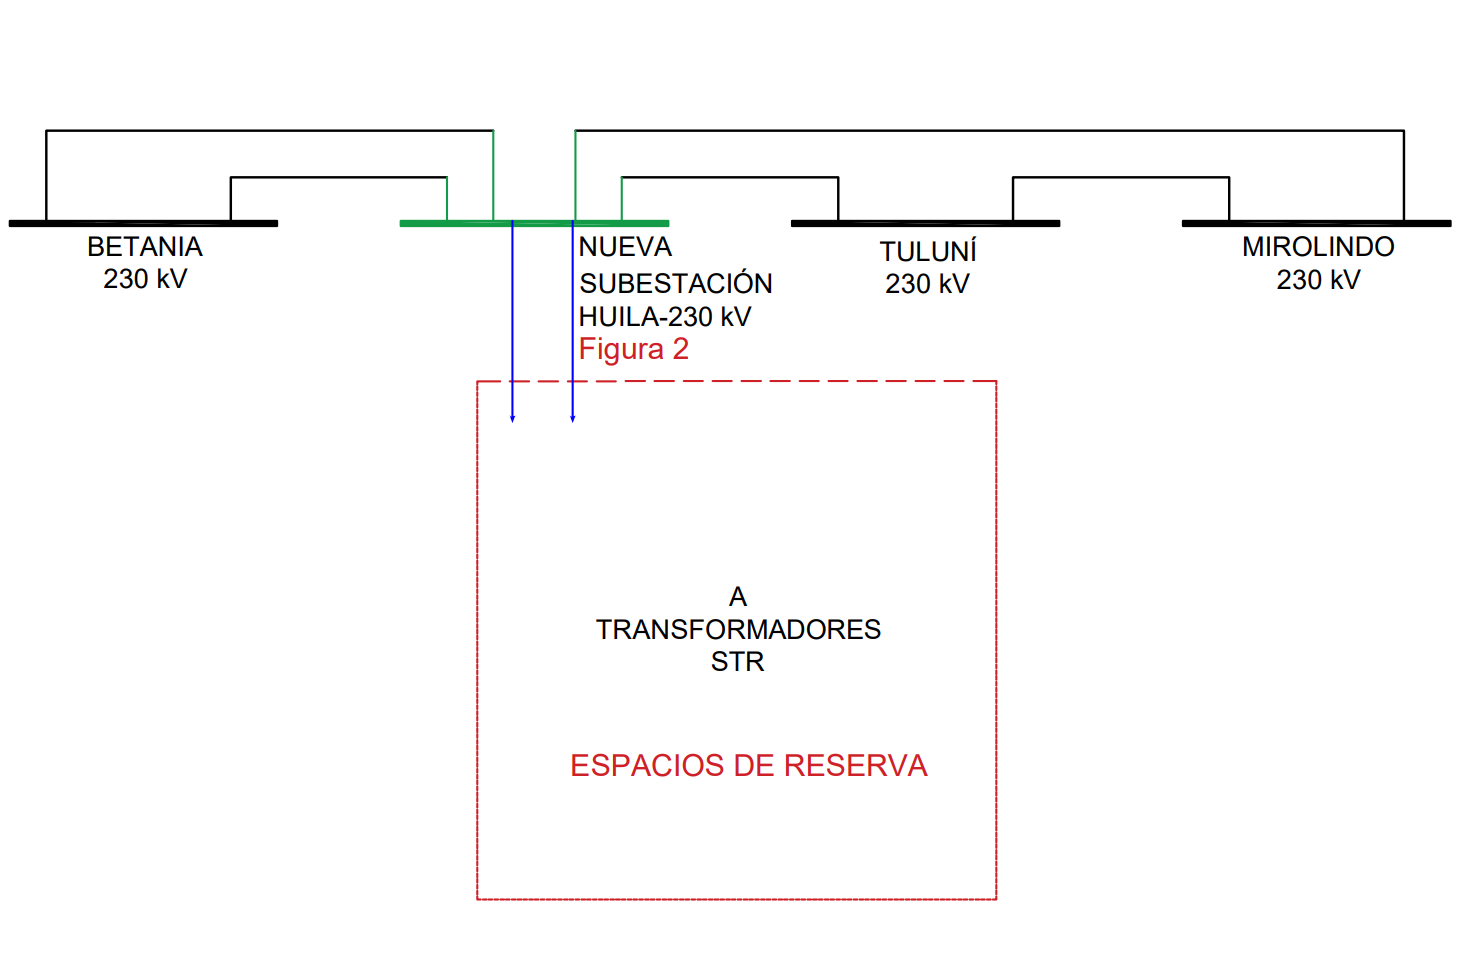
\includegraphics[width=1\textwidth]{1mer avance foticos/Esquema unifilar diagrama esquemático.png}
        \caption{en la figura del diagrama unifilar esquemático como\\ se evidenciará mas adelante en el trazado de la ruta se \\conectará la nueva subestación Huila de dicha forma.} % Título de la figura
        \label{fig:Esquema} % Etiqueta para referencias
    \end{subfigure}
    \hfill % Espacio horizontal entre las subfiguras
    \begin{subfigure}{0.5\textwidth}
        \centering % Centra la imagen
        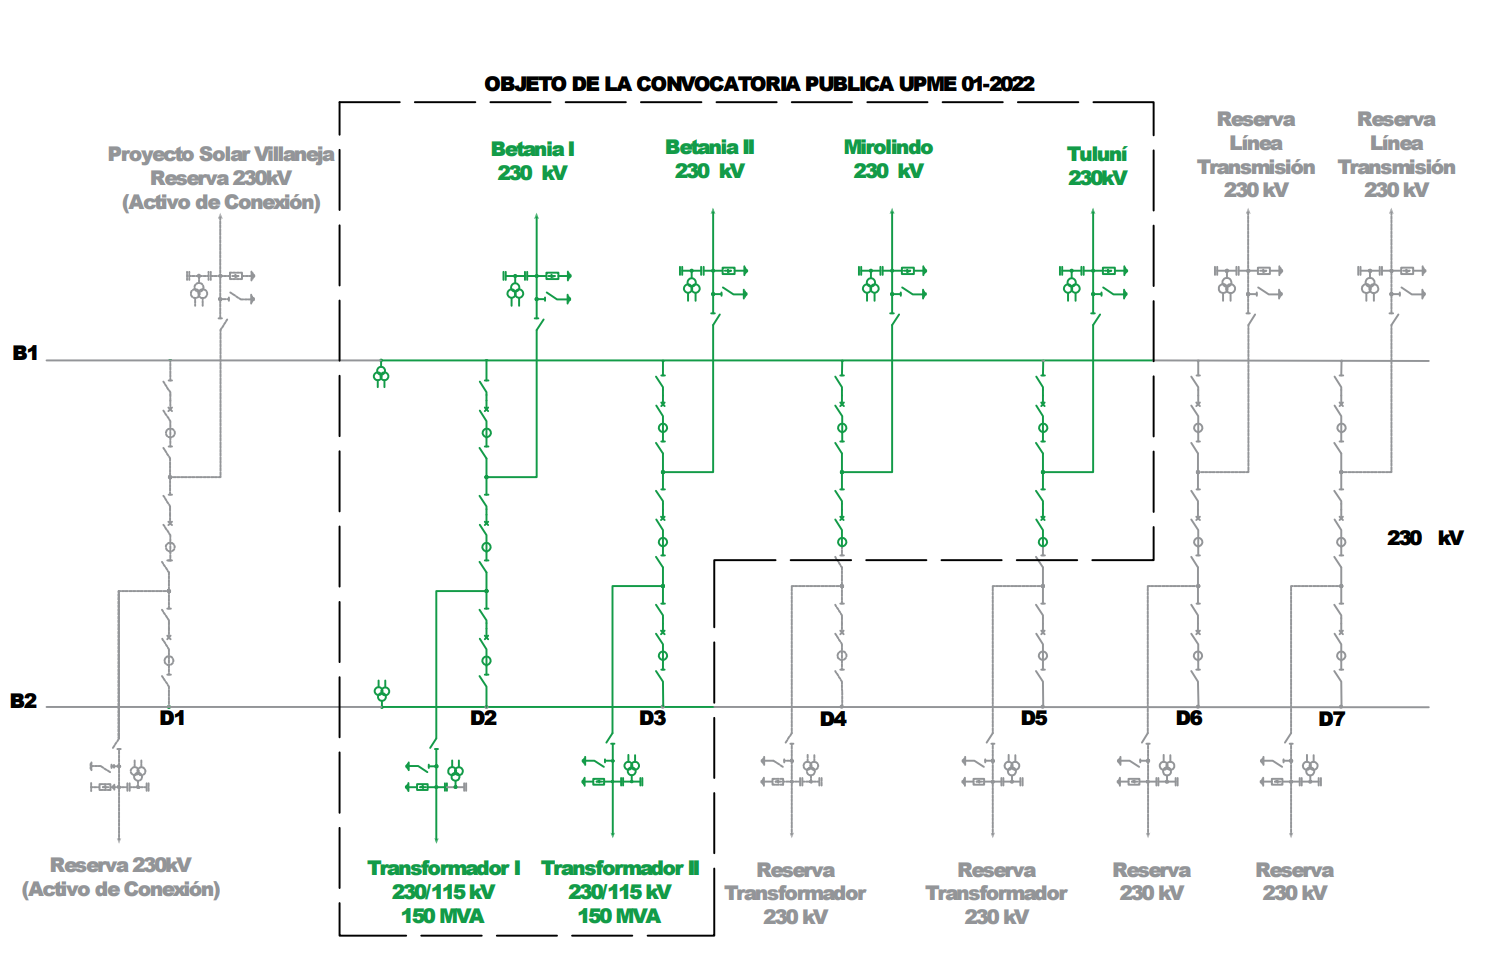
\includegraphics[width=1\textwidth]{1mer avance foticos/Esquema unifilar de la subestación huila 230kv.png}
        \caption{Esquema unifilar de la subestación huila 230kv.} % Título de la figura
        \label{fig:unifilar} % Etiqueta para referencias
    \end{subfigure}
    \label{fig:dos-imagenes}
\end{figure}



%En la \figurename~\ref{fig:unifilar} se muestra un ejemplo de cómo insertar y referenciar imágenes en LaTeX. Este formato permite que, si la imagen se mueve a otra parte del documento, la referencia se actualice automáticamente.


\section{Descripción de los Componentes}

La torre de transmisión analizada corresponde a la torre 002 de la subestación ESSA en Floridablanca, sede Ruitoque Bajo. Se trata de una torre de suspensión con doble circuito y tres fases. Una de las líneas pertenece al circuito Río Frío - Florida, mientras que la otra corresponde al circuito Conucos - Florida, los cuales alimentan distintas zonas del sistema eléctrico.

Los principales componentes son:

\begin{itemize}
    \item \textbf{Circuito eléctrico:} La línea cuenta con un doble circuito.
    \item \textbf{Conductores de fase:} Son los cables principales encargados de transportar la energía eléctrica a alta tensión. Se observan tres fases por circuito, cumpliendo con la configuración estándar.
    \item \textbf{Aisladores:} Se identificaron cadenas de aisladores de suspensión, cuya función es separar eléctricamente los conductores de la estructura metálica de la torre, evitando cortocircuitos y pérdidas de energía.
    \item \textbf{Cable de guarda con conexión a tierra:} Situado en la parte superior de la torre, protege la línea contra descargas atmosféricas (rayos) y disipa la corriente hacia tierra a través del sistema de puesta a tierra.
    \item \textbf{Placa de identificación:} Contiene información sobre la línea, incluyendo el nombre del propietario y los datos técnicos relevantes.
    \item \textbf{Dispositivo antiescalamiento:} Instalado en la base de la torre para evitar accesos no autorizados, contribuyendo a la seguridad del personal y de terceros.
    \item \textbf{Amortiguador de vibraciones:} Se utiliza para reducir las vibraciones eólicas en los conductores de la línea de transmisión. Estas vibraciones son causadas por el viento, lo que puede generar fatiga en el cable y dañarlo con el tiempo.
    \item \textbf{Puesta a tierra:} Su función principal es proteger la estructura y los equipos contra sobretensiones, especialmente descargas atmosféricas.
\end{itemize}

\section{Dimensiones y Distancias de Aislamiento}

Las principales dimensiones y distancias de aislamiento de la estructura son las siguientes:

\begin{itemize}
    \item Distancia mínima de servidumbre: 20 m.
    \item Distancia entre fases: Aproximadamente 2 m.
    \item Distancia al suelo: Aproximadamente 7 m, cumpliendo con los requisitos del RETIE.
    \item Longitud de las cadenas de aisladores: 2 m.
\end{itemize}

\section{Cumplimiento con el RETIE}

Basándonos en la observación y sin realizar mediciones directas, se pueden analizar algunos requisitos del Reglamento Técnico de Instalaciones Eléctricas (RETIE):

\begin{itemize}
    \item \textbf{Distancia de seguridad al suelo:} La separación observada parece cumplir con la normativa, que establece un mínimo de 7 metros en zonas de tránsito restringido.
    \item \textbf{Aisladores y distancias de seguridad:} La longitud de los aisladores y la separación entre fases parecen adecuadas para evitar descargas disruptivas.
    \item \textbf{Sistema de puesta a tierra:} La presencia del cable de guarda sugiere que la torre cuenta con un sistema de protección contra sobretensiones.
    \item \textbf{Identificación y seguridad:} La existencia de una placa de identificación y un dispositivo antiescalamiento indica que la estructura cumple con los requisitos de señalización y seguridad establecidos en el RETIE.
\end{itemize}

%\input{1mer avance maletina.tex}
%
\subsection*{Tabla T2: Resultados para 180 Hz}
Para este caso de frecuencia de muestreo se consiguen valores con un porcentaje de error del 0.0001\% con relación a los datos obtenidos analíticamente, se aprecia que la frecuencia a la que se esta muestreando es 3 veces el valor de la frecuencia fundamental por lo cual no se incumple el teorema de Nyquist-Shannon.
\begin{table}[h!]
    \centering
    \begin{tabular}{@{}ccccc@{}}
        \toprule
        Vrms [Vrms] & Irms [Arms] & P [W] & Q [VAR] & S [VA] \\ \midrule
            110 & 11.0293 & 1155.1 & 371.1589 & 1213.2\\ 
            \bottomrule
    \end{tabular}
    \caption{Resultados medidos a 180 Hz.}
\end{table}



\subsection*{Tabla T2: Resultados para 200 Hz}
Para este caso es posible conseguir valores mas precisos, se requería de tres ventanas de observación de las cuales solo se están usando dos para tomar medidas y además de eso diez medidas de las cuales solo tenemos información de seis en esas dos ventanas de observación.
\begin{table}[h!]
    \centering
    \begin{tabular}{@{}ccccc@{}}
        \toprule
        Vrms [Vrms] & Irms [Arms] & P [W] & Q [VAR] & S [VA] \\ \midrule
        118.8136 & 11.7527 & 1155.1 & 784.6681 & 1396.4 \\ 
        \bottomrule
    \end{tabular}
    \caption{Resultados medidos a 200 Hz.}
\end{table}

\subsection*{Tabla T3: Resultados para 240 Hz}
Para este caso de frecuencia de muestreo se consiguen valores con un porcentaje de error del 0.0001\% exactamente igual a la frecuencia de 180 [Hz]. Con relación a los datos obtenidos analíticamente, se aprecia que la frecuencia a la que se esta muestreando es 4 veces el valor de la frecuencia fundamental por lo cual no se incumple el teorema de Nyquist-Shannon. 

\begin{table}[h!]
    \centering
    \begin{tabular}{@{}ccccc@{}}
        \toprule
        Vrms [Vrms] & Irms [Arms] & P [W] & Q [VAR] & S [VA] \\ \midrule
        110.0000 & 11.0293 & 1155.1 & 371.1590 & 1213.2 \\ 
        \bottomrule
    \end{tabular}
    \caption{Resultados medidos a 240 Hz.}
\end{table}

\subsection*{Tabla T4: Resultados para 280 Hz}
Similar al caso de la frecuencia de 200 Hz para este se requería de catorce muestras de las cuales solo se tienen nueve, además de eso se requería de tres ventanas de observación de las cuales solo se tienen dos.
\begin{table}[h!]
    \centering
    \begin{tabular}{@{}ccccc@{}}
        \toprule
        Vrms [Vrms] & Irms [Arms] & P [W] & Q [VAR] & S [VA] \\ \midrule
        116.6726 & 11.5761 & 1155.1 & 699.9905 & 1350.6  \\ 
        \bottomrule
    \end{tabular}
    \caption{Resultados medidos a 280 Hz.}
\end{table}

\subsection*{Tabla Final: Resultados para 100 Hz}
Finalmente en este caso se da antialiasing, puesto que la frecuencia de muestreo de la señal es menor al doble de la frecuencia fundamental de la red.
\begin{table}[h!]
    \centering
    \begin{tabular}{@{}ccccc@{}}
        \toprule
        Vrms [Vrms] & Irms [Arms] & P [W] & Q [VAR] & S [VA] \\ \midrule
        118.8136 & 13.2088 & 1155.1 & 1062.5 & 1569.4 \\ 
        \bottomrule
    \end{tabular}
    \caption{Resultados medidos a 100 Hz.}
\end{table}
	
%
\section*{Factor de Potencia (FP) y Potencia Activa Consumida por el Parlante}

\begin{table}[h!]
\centering
\begin{tabular}{ccc}
\toprule
\textbf{Frecuencia [Hz]} & \textbf{FP (Factor de Potencia)} & \textbf{($P_{\text{parlante}}$) [W]} \\
\midrule
100  & 0.7361 & 1129.2 \\
180  & 0.9521 & 1129.2 \\
200  & 0.8272 & 1129.2 \\
240  & 0.9521 & 1129.2 \\
280  & 0.8552 & 1129.2 \\
\bottomrule
\end{tabular}
\caption{Resultados de FP y potencia activa consumida por el parlante para diferentes frecuencias.}
\label{table:resultados}
\end{table}

%\section{Modelo del circuito}

Para el circuito de la Figura \ref{fig:mi_imagen} se tiene que la corriente $I$ es la misma en todas las ramas
    

\begin{figure}[h] % 'h' indica que la imagen se coloca aquí
    \centering
    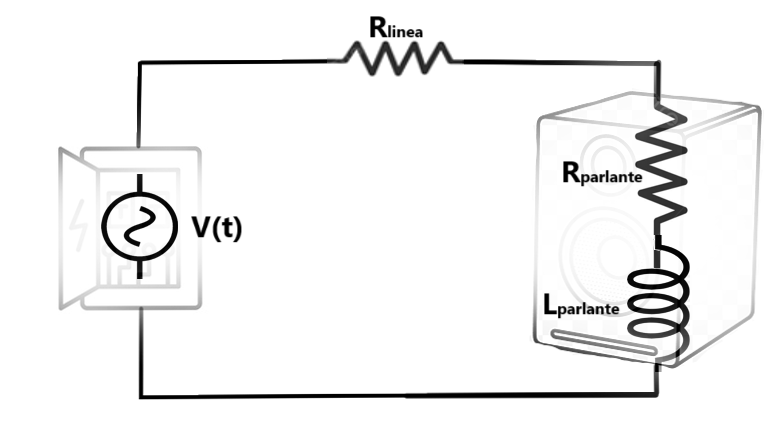
\includegraphics[width=0.5\textwidth]{img/Modelo del circuito.png} % Cambia la ruta a tu imagen
    \caption{Modelo del circuito con el parlante y tablero de Distrubución.}
    \label{fig:mi_imagen}
\end{figure}
%
\section{Porcentajes de Error Para Cada Frecuencia de Muestreo}
A continuacion se presenta el porcentaje de error para cada una de las frecuncias de muestreo.

    \begin{tabular}{ccccc}
        \toprule
        \textbf{Parametro} & \textbf{Error[\%] $f_{\text{100Hz}}$} & \textbf{Error[\%] $f_{\text{180Hz}}$}\\
        \midrule
        Vrms                  & 8.0124   & 0  \\                     
        Irms                  & 19.761  & 0  \\
        P                     & 33.14      & 0  \\
        Q                     & 15.793 & 0 \\
        S                     & 29.36  & 0 \\
        FP                    & 22.68  & 0 \\
        $P_{\text{parlante}}$ & 32.917      & 0  \\
        \bottomrule
        \end{tabular}

    \begin{tabular}{ccc}
        \toprule
        \textbf{Error[\%] $f_{\text{200Hz}}$} & \textbf{Error[\%] $f_{\text{240Hz}}$} & \textbf{Error[\%] $f_{\text{280Hz}}$} \\
        \midrule
        8.0124 & 0 & 6.066 \\ 
        6.5589 & 0 & 4.9577 \\
        16.665 & 0 & 12.492 \\
        1.3999 & 0 & 0.78514 \\
         15.101 & 0 & 11.325 \\
         13.12 & 0 & 10.18 \\
         16.738 & 0 & 12.558   \\
        \bottomrule
        \end{tabular}

%\section{Comparación de procesos de muestreo}
    Para los casos en los cuales se emplearon frecuencias de muestreo de 240 Hz y 180 Hz son los mas eficaces puesto que solo emplean una sola ventana de observación para realizar la estimación de los parámetros de la señal, en cambio en las señales de 280 Hz y 200 Hz se realizan de otra ventana de observación incluyendo las dos en las que se tomo la medición además requerían de 5 y 4 medidas adicionales respectivamente.\\ 

\section{Relación con el Teorema de Nyquist-Shannon}
El teorema de Nyquist-Shannon establece que, para evitar el aliasing y permitir la reconstrucción perfecta de una señal, la frecuencia de muestreo debe ser al menos el doble de la frecuencia máxima de la señal.
\begin{equation}
    f_s \geq 2 f_{\text{máx}}
\end{equation}

\section{Conclusiones y Recomendaciones}
La frecuencia de muestreo tiene un impacto significativo en la estimación de parámetros en sistemas eléctricos. La correcta elección de esta frecuencia, fundamentada en el teorema de Nyquist-Shannon, asegura que la información crítica de la señal sea capturada de manera precisa y que se minimicen los efectos del aliasing. En conclusión, para obtener mediciones confiables y precisas, es esencial seleccionar una frecuencia de muestreo que no solo cumpla con la condición de Nyquist, sino que también considere la naturaleza y dinámica del sistema en estudio.


\end{document}  
